\documentclass[12pt]{book}
\usepackage[utf8]{inputenc}
\usepackage{minted}
\usepackage{multirow}
\usepackage{listings}

\usepackage{amssymb,amsmath,amsthm,amsfonts}
\usepackage{calc}
\usepackage{graphicx}
\usepackage{subfigure}
\usepackage{indentfirst}
\usepackage{titlesec}
%\newcommand{\sectionbreak}{\clearpage}
\DeclareGraphicsExtensions{.bmp,.png,.pdf,.jpg}
\usepackage{gensymb}

\usepackage{url}
\usepackage{amsmath}
\usepackage{graphicx}
\graphicspath{{images/}}
\usepackage{parskip}
\usepackage{fancyhdr}
\usepackage{vmargin}
\setmarginsrb{2 cm}{2 cm}{2 cm}{2 cm}{1 cm}{1.5 cm}{1 cm}{1.5 cm}

\lstdefinelanguage{Marlowe}{%
  language     = Haskell,
  morekeywords = {Close, Pay, Assert, If, When, Let},
}
\lstdefinelanguage{Isabelle}{%
  language     = ML,
  morekeywords = {theory, imports, begin, end},
}

\definecolor{codegreen}{rgb}{0,0.6,0}
\definecolor{codegray}{rgb}{0.5,0.5,0.5}
\definecolor{codepurple}{rgb}{0.58,0,0.82}
\definecolor{backcolour}{rgb}{0.95,0.95,0.92}

\lstdefinestyle{Haskell-cardano}{
    backgroundcolor=\color{backcolour},   
    commentstyle=\color{codegreen},
    keywordstyle=\color{magenta},
    numberstyle=\tiny\color{codegray},
    stringstyle=\color{codepurple},
    basicstyle=\ttfamily\footnotesize,
    breakatwhitespace=false,         
    language=Haskell,
    breaklines=true,                 
    captionpos=b,                    
    keepspaces=true,                 
    numbers=none,                    
    numbersep=5pt,                  
    showspaces=false,                
    showstringspaces=false,
    showtabs=false,                  
    tabsize=2
}

\definecolor{isarblue}{HTML}{006699}
\definecolor{isargreen}{HTML}{009966}
\lstdefinelanguage{isabelle}{%
    keywords=[1]{type_synonym,datatype,fun,abbreviation,definition,proof,lemma,theorem, theory,corollary},
    keywordstyle=[1]\bfseries\color{isarblue},
    keywords=[2]{where,assumes,shows,and, imports, begin, end},
    keywordstyle=[2]\bfseries\color{isargreen},
    keywords=[3]{if,then,else,case,of,SOME,let,in,O},
    keywordstyle=[3]\color{isarblue},
}
\lstdefinestyle{Isabelle}{%
  language=isabelle,
  escapeinside={&}{&},
  columns=fixed,
  extendedchars,
  frame=single,
  basewidth={0.5em,0.45em},
  basicstyle=\ttfamily,
  mathescape,
}



\usepackage[spanish]{babel}
\usepackage[colorlinks=true, allcolors=blue]{hyperref}
\hypersetup{
    colorlinks=true,% make the links colored
}
\usepackage[nolist]{acronym}
\usepackage[table]{xcolor}
\usepackage{url}

%% Biblatex
%\usepackage[style=plain]{biblatex}
%\addbibresource{bibliografia.bib}

\begin{document}

\begin{titlepage}

\title{     \textbf{Tesis de Grado \\ de Ingeniería en Informática}\\[2.5ex]
\textit{Verificación de smart contracts en Marlowe\\ para la blockchain Cardano}}

\author{
             \textbf{Director:} Dr. Ing. Mariano G. Beiró \\
         \texttt{mbeiro@fi.uba.ar}\\[2.5ex]
             \textbf{Co-director:} Phd. Simon Thompson (Kent University, IOHK) \\
         \texttt{S.J.Thompson@kent.ac.uk}
             \\[2.5ex]
             \textbf{Alumno:} Julián Ferres, \textit{(Padrón \#101.483)}                                \\
                    \texttt{ jferres@fi.uba.ar }                                    \\[2.5ex]
            \normalsize{Facultad de Ingeniería, Universidad de Buenos Aires}        \\
       }
\date{\today}

\end{titlepage}

\maketitle
\thispagestyle{empty}

\maketitle

{
  \hypersetup{linkcolor=black}
  \tableofcontents
}

%  Capitulos
%  1) Introducción (concepto de blockchain, aplicaciones, IOHK, Ada, Plutus) (8 a 10 páginas)
%  2) Escritura de contratos financieros en Marlowe para Cardano (15 a 20 páginas)
%     a. Marlowe como DSL
%     b. El estándar ACTUS
%  3) Verificación de programas (12 a 15 páginas)
%     a. Concepto general, herramientas, metodologías
%     b. Isabelle
%  4) Desarrollo: verificación de contratos financieros usando Isabelle (30 páginas)
%     a. Escritura de contratos Actus para Cardano
%     b. sss
%     c. sss
%  5) Conclusión (3 páginas)
%  6) Bibliografía (4 páginas)
%  7) Apéndice (código)



%##########################
% INTRODUCCIÓN
%##########################

\chapter{Introducción}

%##########################
% Escritura de contratos financieros en Marlowe para Cardano
%##########################

\chapter{Escritura de contratos financieros en Marlowe para Cardano}
\section{Marlowe como DSL}
Marlowe \cite{implementing_financial_contracts_on_blockchain}, \cite{standardized_crypto_loans} es un lenguaje pequeño, con pocas sentencias soportadas que, para cada contrato, describen el comportamiento que involucra un conjunto fijo y finito de roles.

Marlowe está diseñado para crear bloques para contratos financieros: pagos o depósitos de las partes, elecciones e información del mundo real. Cuando se ejecuta un contrato, los roles que implica son satisfechos por los participantes, que son identidades en la cadena de bloques. Cada rol está representado por un token en la cadena y los roles se pueden transferir durante la ejecución del contrato, lo que significa que esencialmente se pueden intercambiar.

Los contratos se pueden construir reuniendo una pequeña cantidad de estas sentencias que, en combinación, se pueden usar para describir y modelar muchos tipos diferentes de contratos financieros. Algunos ejemplos incluyen un contrato que puede realizar un pago a un rol o a una clave pública, un contrato que puede esperar una acción por parte de uno de los roles, como un depósito de moneda, o una elección entre un conjunto de opciones.

En particular, un contrato no puede esperar indefinidamente una acción: si no se ha realizado en un tiempo determinado (conocido como \textit{timeout}), el mismo continuará con un comportamiento alternativo, por ejemplo, reembolsar los fondos en el contrato.

Los contratos de Marlowe pueden ramificarse en función de alternativas y tienen una vida finita, al final de la cual el dinero restante retenido por el mismo se devuelve a los participantes. Esta característica garantiza que el dinero no se puede bloquear para siempre en un contrato. Dependiendo del estado actual de un contrato, puede elegir entre dos cursos de acción alternativos, que son en sí mismos contratos. Cuando no se requieran más acciones, el contrato se cerrará y se reembolsará cualquier moneda restante en el contrato.

\subsection{Contratos en Marlowe}
Un contrato en Marlowe se obtiene combinando una pequeña cantidad de sentencias o \textit{building blocks}. Las mismas pueden llegar a describir muchos tipos de contratos financieros, como hacer un pago, hacer una observación, esperar hasta que cierta condición se cumpla, etc. Luego, el contrato se ejecuta en una cadena de bloques, como Cardano, e interactúa con el mundo exterior.

Marlowe, en sí mismo, está embebido en Haskell y se modela como una colección de tipos de datos algebraicos en Haskell \textcolor{red}{(alguna referencia sobre el concepto de tipo de dato algebraico)}, con contratos definidos por el tipo de contrato:

\begin{lstlisting}[language=Marlowe]
data Contract = Close
              | Pay Party Payee Token Value Contract
              | If Observation Contract Contract
              | When [Case] Timeout Contract
              | Let ValueId Value Contract
              | Assert Observation Contract
\end{lstlisting}

Marlowe tiene seis maneras de construir contratos. Cinco de esos métodos – 
\texttt{Pay}, \texttt{Let}, \texttt{If}, \texttt{When}, and \texttt{Assert} - construyen un contrato complejo a partir de contratos más simples, y el ultimo método, \texttt{Close} es un contrato simple. En cada paso de la ejecución, además de modificar el estado y proceder hacia un nuevo contrato, podrían generarse pagos y advertencias (\textit{warnings}).

Antes de describir los métodos exhaustivamente, es útil conocer la definición de valores, observaciones y acciones:

\begin{itemize}
    \item \textbf{Valores}: Incluyen cantidades que cambian con el tiempo, tales como: el \textit{slot interval} o 'intervalo actual', el balance de cierto token en una cuenta o elecciones que se han realizado (conocidas como \textit{valores volátiles}). Los valores pueden ser combinados usando operaciones como suma, resta, negación, etc. Los mismos pueden ser valores condicionales o una observación.
    
    \item \textbf{Observaciones}: Valores booleanos que son obtenidos al comparar valores, y que pueden ser combinados con los operadores booleanos estándar. Además, es posible observar si alguna elección se ha realizado (para una elección en concreto). Las observaciones tendrán un valor en cada etapa de la ejecución.
    
    \item \textbf{Acciones}: Suceden en momentos particulares durante la ejecución, por ejemplo: un depósito de dinero o elegir entre varias alternativas.
    
    % Revisar oracles, que parecen haber sido incluidos, pero no estoy seguro de si son relevantes o no para nuestro trabajo.

\end{itemize}


\subsubsection{Pay}
Un contrato de pago \texttt{(Pay acc payee tok val cont)} realizará un pago de valor \texttt{val} de un token \texttt{tok} desde una cuenta \texttt{acc} a un beneficiario \texttt{payee}, quien sera uno de los participantes del contrato, u otra cuenta en el mismo.

Se generarán \textit{warnings} si el valor \texttt{val} no es positivo, o si no hay recursos suficientes en \texttt{acc} para realizar el pago en su totalidad (incluso si hay balances positivos de otros tokens en la misma). En este último caso, se realizará un pago parcial (conteniendo todo el dinero disponible). El contrato en el que continuará la ejecución es \texttt{cont}.

\subsubsection{Close}

Un contrato \texttt{Close} prevé que el contrato sea cerrado (o rescindido). La única acción que realiza es reembolsar a los titulares de cuentas que contienen un saldo positivo. Esto se realiza de a una cuenta a la vez, pero todas las cuentas se reembolsarán en una sola transacción.

\subsubsection{If}
El conditional \texttt{If obs cont1 cont2} continuará en \texttt{cont1} o \texttt{cont2}, dependiendo de la observación \texttt{obs} cuando el mismo es ejecutado.

\subsubsection{When}
Es el constructor de contratos mas complejo, con la forma \texttt{When cases timeout cont}. El mismo es activado por acciones, que pueden o no ocurrir en un \textit{slot} en particular. Como continua el mismo tras una acción se declara en la sintaxis de \texttt{cases} del contrato.

En el contrato \texttt{When cases timeout cont}, la lista \texttt{cases} contiene una colección de casos. Cada caso es de la forma \texttt{Case ac co} donde \texttt{ac} es una acción y \texttt{co} un contrato de continuación. Cuando una acción en particular, por ejemplo \texttt{ac}, ocurre, el estado del contrato es actualizado correspondientemente y y mismo continuara su ejecución en \texttt{co}.

Para garantizar que el contrato eventualmente progresará, la ejecución de \texttt{When cases timeout cont} continuará como \texttt{cont} una vez que el slot \texttt{timeout} es alcanzado.

\subsubsection{Let}

Un contrato \texttt{Let id val cont} permite registrar un valor, en un punto particular en el tiempo, y darle nombre usando un identificador. En este caso, la expresión \texttt{val} se evalúa y se almacena con el nombre \texttt{id}. El contrato entonces continúa como \texttt{cont}.

Además de permitirnos usar abreviaturas, este mecanismo nos brinda la capacidad de capturar y guardar valores volátiles que pueden cambiar con el tiempo, por ejemplo: '\textit{el precio actual del petróleo}', '\textit{el slot actual, en un punto particular de la ejecución del contrato}', para ser utilizado más adelante en la ejecución del mismo.

\subsubsection{Assert}
Un contrato \texttt{Assert obs cont} no tiene ningún efecto en el estado de un contrato, que continua inmediatamente en \texttt{cont}, pero genera una advertencia cuando la observación \texttt{obs} es falsa. Puede ser utilizado para asegurar que alguna propiedad se cumple en un momento particular de la ejecución del contrato. Esta sentencia es útil porque permite que un \textit{análisis estático} detecte que algún \texttt{assert} es falso, para alguna ejecución específica del contrato.


\section{El estándar ACTUS}
Los contratos financieros son acuerdos legales entre dos (o más) partes sobre el futuro intercambio de dinero. Dichos acuerdos legales se definen sin ambigüedades por medio de un conjunto de términos y lógica contractual. Como resultado, los mismos pueden describirse matemáticamente y representarse digitalmente como algoritmos. Los beneficios de representar contratos financieros de esta forma son múltiples; Tradicionalmente, el procesamiento de transacciones ha sido un campo en el que se pueden lograr mejoras de eficiencia mediante la automatización de contratos. 

Adicionalmente, el análisis financiero (por naturaleza del dominio) se basa en la disponibilidad de representaciones computables de estos acuerdos, donde a menudo se utilizan aproximaciones analíticas. Recientemente, el auge de las blockchain, de contabilidad distribuida y los diversos casos de uso de los contratos inteligentes han abierto nuevas posibilidades para los contratos financieros digitales.

En general, el intercambio de flujos de efectivo entre partes sigue ciertos patrones. Un patrón típico es un contrato de préstamo de tipo \textit{bullet}, donde un monto de dinero inicial se entrega, a cambio de pagos de intereses cíclicos y la devolución del dinero inicial en el vencimiento del contrato. Si bien los pagos son fijos, existen muchas variantes que determinan cómo se programan y/o pagan los pagos de intereses cíclicos. Por ejemplo, los pagos de intereses pueden ser mensuales, anuales, mediante períodos arbitrarios. Pueden además ser de tasa fija o variable, pueden usarse diferentes métodos de cálculo de fracciones anuales o puede que no haya ningún interés.

Otro patrón popular es el de amortización de préstamos, en el que, a diferencia de los préstamos \textit{bullet}, el dinero inicial prestado puede devolverse en porciones de montos fijos o variables, y de acuerdo con cronogramas cíclicos o personalizados. Otros tipos de contratos financieros a mencionar incluyen, acciones, contratos a plazo, opciones, swaps, mejoras crediticias, acuerdos de recompra, titularización, etc. 

Al centrarse en las principales características distintivas, ACTUS describe la gran mayoría de todos los contratos financieros con un conjunto de alrededor de 32 patrones generales de flujo de efectivo, también conocidos como 'tipos de contrato'.

La taxonomía ACTUS~\cite{ACTUS_Taxonomy}  proporciona un sistema de clasificación que organiza los contratos financieros según sus patrones distintivos de flujo de dinero. Aparte de este sistema de clasificación, la taxonomía también incluye una descripción de los instrumentos del mundo real cubiertos por cada contrato. 
 
Por otro lado, los acuerdos legales en los contratos financieros representan una lógica puramente determinista. Es decir, un contrato financiero define un conjunto fijo de reglas y condiciones bajo las cuales, dado cualquier conjunto de variables externas, las obligaciones de flujo de efectivo pueden determinarse sin ambigüedades. Por ejemplo, en un préstamo de tasa fija, las obligaciones de flujo de efectivo se definen explícitamente. 

Las propiedades de los contratos financieros descritos anteriormente sientan las bases para una descripción algorítmica estandarizada y determinista de las obligaciones de flujo de dinero que surgen de tales acuerdos. Por lo tanto, esta descripción es agnóstica de la tecnología y es compatible con todos los casos de uso necesarios para que este mismo estándar se utilice en todas las funciones financieras. Entre estas se podrían mencionar: fijación de precios, creación de acuerdos, procesamiento de transacciones, así como el análisis en general, proyecciones de liquidez, valoración, cálculos y proyecciones de pérdidas y ganancias, y medición y agregación de riesgos, etc.

Adicionalmente, este estándar crea una base formidable para las máquinas de estados financieras y los \textit{smart contracts}. En la documentación técnica \cite{ACTUS_Techspecs} es posible encontrar la descripción matemática de los contratos financieros. 


\subsection{Notación ACTUS}

Antes de adentrarnos en la especificación de un contrato, es necesario poder entender algunos aspectos de la notación del mismo:

\begin{itemize}
    \item \textbf{Atributos de contrato}: Representan los términos contractuales que definen el flujo de dinero en un contrato financiero. Estos atributos están definidos en \cite{ACTUS_Dictionary_Terms}.
    
    \item \textbf{Starting date}: $t_0$ representa la fecha de comienzo del contrato, y marca el instante en el cual las condiciones y estado del contrato esta siendo representado. En general, partiendo desde la lógica contractual, se podrán determinar los eventos del contrato y el estado para todo $t > t_0$, pero no para $s < t_0$
    
    \item \textbf{Variables de estado}: Las variables de estado describen el estado de un contrato, para un tiempo determinado de su ciclo de vida. Algunos ejemplos de las mismas son: \textit{Notional Principal}, \textit{Nominal Interest Rate}, o \textit{Contract Performance}. 
    
    El diccionario de ACTUS \cite{ACTUS_Dictionary_States} define todas las variables de estado y provee información adicional sobre el tipo de dato esperado por cada una, el formato, etc. 
    
    En general, el 'estado' representa ciertos términos de un contrato que pueden cambiar a lo largo de su ciclo de ejecución, de acuerdo a eventos programados o no programados. Las variables están escritas en su forma abreviada con la primera letra en mayúscula, en negrita e indexadas mediante el tiempo.
    
    \item \textbf{Eventos}: Un evento de contrato (o simplemente evento) $e^k_t$ se refiere a cualquier evento programado o no programado en un momento determinado $t$ y de un tipo determinado $k$. 
    
    Los eventos del contrato marcan puntos específicos en el tiempo (durante la ejecución del mismo) en el que se intercambian flujos flujo de efectivo o se actualizan los estados del contrato. El diccionario de eventos \cite{ACTUS_Dictionary_Events} enumera y describe todos los tipos de eventos $k$ definidos por los estándares ACTUS.
    
    \item \textbf{Funciones de transición de estado} Dichas funciones, conocidas en Inglés como \textit{'State Transicion Functions'} (STF) definen la transición de las variables de estado desde el \textit{pre-evento} hacia el \textit{post-evento}, cuando un cierto evento $e^k_t$ ocurre. Esto provoca que el  \textit{pre-evento} y \textit{post-evento} reciban la notación de $t^-$ y $t^+$ respectivamente.
    
    Estas funciones son específicas para un tipo de evento y contrato. Las mismas son escritas de acuerdo al siguiente formato $\textbf{STF\_[event type]\_[contract type]()}$, donde $\text{[event type]}$ y $\text{[contract type]}$ hacen alusión al tipo de evento y contrato al cual la STF pertenece. 
    
    Por ejemplo: La STF para un evento de tipo IP en el contrato PAM se escribe como $\text{STF\_IP\_PAM()}$ y modifica (entre otras) a la variable $\textbf{Ipac}$ desde el pre-evento $\textbf{Ipac}_{t^-}$ al post-evento $\textbf{Ipac}_{t^+}$.
    
    \item \textbf{Funciones de pago}: Las funciones de pago, o Payoff Functions (POF) definen como el flujo de dinero $c \in \mathbb{R}$ ocurre para un determinado evento $e^k_t$. El mismo es obtenido del estado actual y los terminos del contrato. Si fuera necesario, el flujo de dinero puede ser indexado con el tiempo del evento: $c_t$. 
    
    Las funciones de pago (de forma analoga a las STF), son específicas para un tipo de evento y contrato, y su notación es la siguiente: $\textbf{POF\_[event type]\_[contract type]()}$, donde $\text{[event type]}$ y $\text{[contract type]}$ hacen alusión al tipo de evento y contrato al cual la POF pertenece. 

    Por ejemplo: La POF para un evento de tipo IP $e^{IP}_t$ en el contrato PAM se escribe como $\text{POF\_IP\_PAM()}$.

    \item \textbf{Fechas/Tiempo}: Sin adentrarnos demasiado en particularidades, cabe aclarar que ACTUS utiliza el formato de fechas ISO 8601. Por lo tanto, las fechas son usualmente expresadas en el siguiente formato: [YYYY]-[MM]-[DD]T[hh]:[mm]:[ss]. El formato no soporta husos horarios.
    
    \item \textbf{Secuencia de eventos}: Los eventos (de diferentes tipos) de un contrato pueden ocurrir en el mismo instante de tiempo $t$. En este caso, la secuencia de evaluación de su $STF$ y $POF$ es crucial para los flujos de efectivo resultantes y las transiciones de estado. Por lo tanto, se utiliza un indicador de secuencia de eventos que se puede encontrar para cada evento en el diccionario de eventos. Este implica el orden de ejecución de  diferentes eventos en el mismo tiempo $t$.
    
    \item \textbf{Lifetime de contrato}: La vida útil de un contrato ACTUS es el período de tiempo de su existencia, desde la perspectiva del usuario que analiza. Para cada punto en el tiempo durante su vida, se puede analizar un contrato ACTUS en términos de estado actual y flujos de efectivo futuros.
    
\end{itemize}

\subsection{Un contrato de ejemplo}

% Usar \href{https://github.com/actusfrf/actus-techspecs/blob/master/actus-techspecs.tex}{TeX de la especificación ACTUS} para sacar alguna captura de pantalla, o ver si es posible embeber alguna de sus tablas en este manuscrito. 
% UPD: Me ha resultado imposible hacerlo (al menos con mis conocimientos de latex actuales, debido a que ellos usan un tipo especial de documento que pareciera llevarse mejor con tablas que el nuestro. Por lo pronto solo incluiré imagenes relevantes de parte de las tablas

En esta sección, recorreremos brevemente la especificación técnica ofrecida por ACTUS \cite{ACTUS_Techspecs}. En particular, nos centraremos en un tipo de contrato llamado \textit{Principal at Maturity} (PAM).

El propósito del contrato PAM puede ser resumido en el siguiente párrafo:

\textit{'Se efectuará un pago del valor total en la fecha de intercambio inicial (simbolizada con la variable de contrato IED) y es reembolsado en la fecha de vencimiento (MD). Dependiendo de las variables de contrato, podrían aplicarse tarifas fijas o variables.'}

Al describir el contrato, la especificación técnica separa al mismo en tres tablas. Las mismas expresan de forma declarativa, que acción debe ocurrir ante determinado evento. 

Las filas de las tablas representan los diferentes tipos de eventos que el contrato tolera, y en las columnas se encuentra la acción correspondiente, junto con comentarios apropiados:

\begin{itemize}
    \item \textbf{Contract Schedule (Cronograma del contrato)}: Contiene información acerca de los eventos programados para dicho contrato. En general, se realiza la asignación a las variables de estado correspondiente. Dichas variables reciben fechas o vectores de fechas (en caso de que el tipo de evento pueda ocurrir en múltiples instantes de la vida del contrato). 
    
    Por ejemplo, para el evento de \textit{monitoring} (AD), un contrato podría definir $\vec{t}^{AD} = \left(t_0,t_1, \ldots ,t_n\right)$, siendo $t_1, \ldots, t_n$ tiempos definidos por el usuario.
    
    \item \textbf{State Variables Initialization (Inicialización de variables de estado)}: Esta tabla contiene información acerca del estado inicial de las variables del contrato. Muchas variables son simplemente extraídas de los términos del contrato, mientas que otras tienen estructuras condicionales en su definición.
    
    Dichas variables serán luego utilizadas para definir pagos y funciones de transición de estado.
    
    \item \textbf{State Transition Functions and Payoff Functions (Funciones de transición de estado y de pago)}:
    Esta tabla reune las funciones de transición y de pago correspondientes a un contrato, para cada tipo de evento.
    
    
\end{itemize}


A continuación, se muestran fragmentos de las 3 tablas para el contrato, extraídos de la especificación:

\begin{figure}
    \centering
    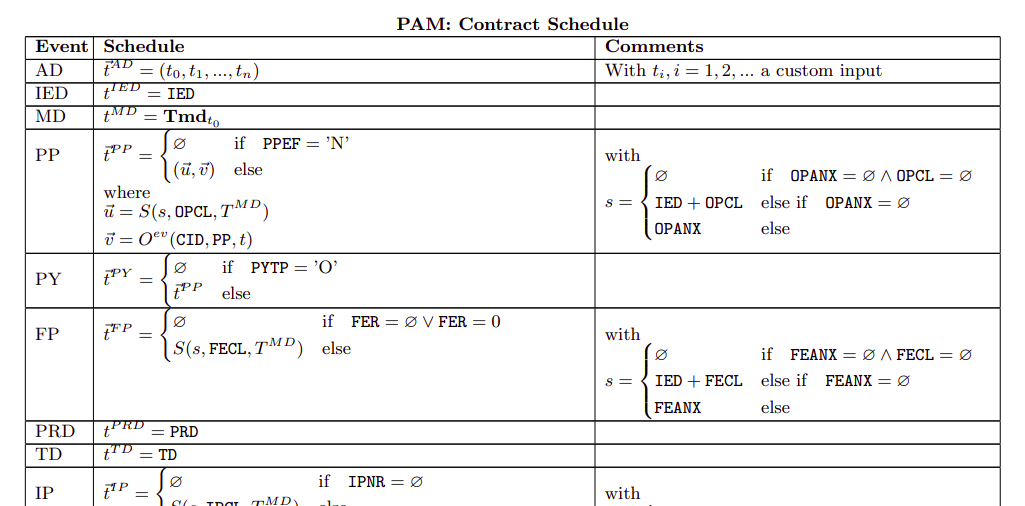
\includegraphics[width=\textwidth]{PAM_Contract_Schedule.png}
    \caption{Cronograma del contrato PAM para algunos eventos}
    \label{fig:PAM_Contract_Schedule}
\end{figure}

\begin{figure}
    \centering
    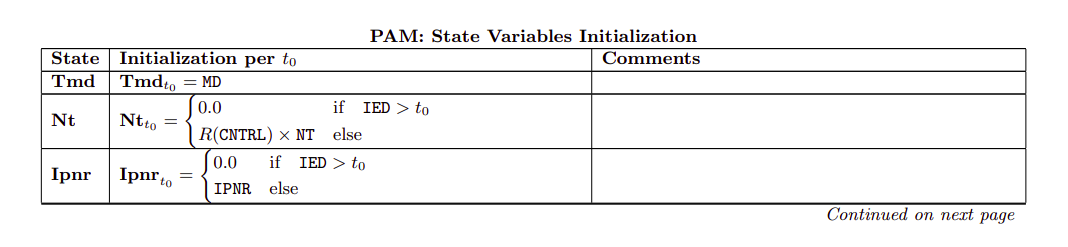
\includegraphics[width=\textwidth]{PAM_State_Variables_Initialization.png}
    \caption{Inicialización de algunas variables del contrato PAM}
    \label{fig:PAM_State_Variables_Initialization}
\end{figure}

\begin{figure}
    \centering
    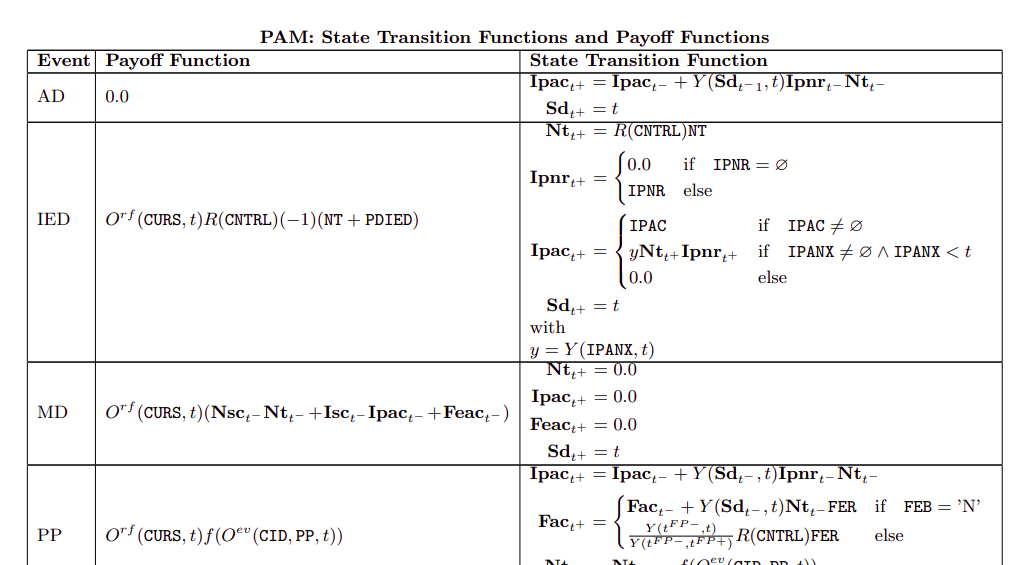
\includegraphics[width=\textwidth]{PAM_STF_POF.png}
    \caption{Funciones de cambio de estado y pago del contrato PAM}
    \label{fig:my_label}
\end{figure}




%##########################
% Verificación de programas
%##########################

\chapter{Verificación de programas}
\section{Concepto general, herramientas, metodologías}
\section{Isabelle}

%##########################
% Desarrollo: verificación de contratos financieros usando Isabelle
%##########################

\chapter{Desarrollo: verificación de contratos financieros usando Isabelle}
\section{Escritura de contratos ACTUS para Cardano}
\section{sss}
\section{sss}

%##########################
% Conclusión
%##########################

\chapter{Conclusión}

%##########################
% Apéndice
%##########################

\chapter{Apéndice}

%##########################
% Bibliografía
%##########################

\bibliographystyle{apalike}
\bibliography{bibliografia.bib}



\end{document}